
\documentclass{beamer}

\usepackage[utf8]{inputenc}

\usepackage[T1]{fontenc}

\usepackage{float}
\restylefloat{table}

\usepackage[english]{babel}

%\usepackage{setspace}
%\doublespacing

\usepackage{amsfonts}
\usepackage{amsmath}

% for lucid chart images
\usepackage{graphicx}

\begin{document}

\begin{frame}
	
\end{frame}

\begin{frame}
	\frametitle{Nash Equilibrium}
	Let $G$ be a game with $K$ players. For each player $k$ we have
	\begin{itemize}
		\item action set $A_k$ of actions available to $k$
		\item strategy set $\Delta(A_k)$ of distributions over actions in $A_k$.
		\item payoff function $\mu_k: \Pi_{i=1}^K A_i \longrightarrow \mathbb{R}$
		\begin{itemize}
			\item payoffs for mixed strategy $p_k \in \Delta(A_k)$: $\underset{a_k \sim p_k}{E}\lbrack \mu_k(\textbf{a}) \rbrack$
		\end{itemize}
	\end{itemize}
	
	A \textbf{Nash Equilibrium} $S$ is a strategy assignment $(p_1,..., p_K)$ such that for each player $k$:
	\begin{equation}
	\forall q \in \Delta(A_k): \mu_k(p_k, S_{-k}) \ge \mu_k(q, S_{-k})
	\end{equation}
	
\end{frame}

\begin{frame}
	\frametitle{$n$-round Prisoner's Dilemma}
	\begin{table}[H]
		\centering
		\label{pdpayoffs}
		\begin{tabular}{lll}
			& C                        & D                        \\ \cline{2-3} 
			\multicolumn{1}{l|}{C} & \multicolumn{1}{l|}{3,3} & \multicolumn{1}{l|}{0,4} \\ \cline{2-3} 
			\multicolumn{1}{l|}{D} & \multicolumn{1}{l|}{4,0} & \multicolumn{1}{l|}{1,1} \\ \cline{2-3} 
		\end{tabular}
	\end{table}
	
	\begin{itemize}
		\item The elements of the action set $A^n_k$ are of the form $\lbrace C,D \rbrace^n$
		\item Backwards induction shows the only Nash equilbrium is $(D^n, D^n)$
	\end{itemize}
	
	% go through backwards induction argument
	
\end{frame}

\begin{frame}
	\frametitle{Questions}
		\begin{itemize}
			\item How can we quantify strategic complexity?
			\item Can we avoid the $(D^n, D^n)$ equilibrium by limiting strategic complexity?
			\item Will players use far more complex strategies for only marginally greater payoffs?
		\end{itemize}
\end{frame}

\begin{frame}
	\frametitle{Bounded Rationality}
	\textbf{implementation complexity}: the number of states required by a finite automaton which implements the strategy	
	
	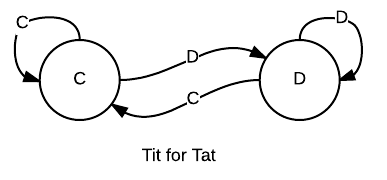
\includegraphics[scale=0.5]{tit4tat}
	
	% for instance: an automaton with less than $n$ states can't count down from $n$ and so our backwards induction argument doesn't work. in fact two automatons with less than $n$ states are in equilbrium each playing tit4tat
	
	\noindent \textbf{Theorem:} Let $\epsilon > 0$ and $G$ an $n$-round Prisoner's Dilemma played by automata. If one of the automata has less than $2^{c_\epsilon n}$ states, then there is a mixed equilibrium with expected payoff for each player at least 3 - $\epsilon$.
	
	% theorem 1 is surprising because there are many more states than rounds and so backwards induction seems to be enabled. furthermore one player may have a arbitrarily larger automata than the other
	
	% should also mention implementation vs selection complexity
\end{frame}

\section{Rational Learning Leads to Nash Equilibrium}

\begin{frame}
	
\end{frame}

\end{document}